%% Section that includes the experiments performed.

This section describes the accomplished experiments that prove how the developed system fulfills SKA's requirements for the PPS distribution system. The first experiment is a general characterization of the developed platform. The second one, tests the equipment in a realistic network topology to evaluate the performance in a possible deployment. The last experiments evaluates the influence of some typical events, such as traffic, temperature fluctuation or \textcolor{blue}{something else} in a network deployment using the WR-ZEN.

Performance of the new WR platform is measured using multiple equipment, and obtained results have been compared to WRS's performance because of it's electronic design is considered as \ftglnote{en serio?}reference for WR technology. The list of the equipment and materials used for the experiments is the following:

\begin{itemize}
    \item Three White Rabbit Switches to simulate a typical WR network. All of them have hardware version 3.4 and 5.0 of firmware.
    \item A White Rabbit ZEN Time Provider (WR-ZEN TP) to test the performance of the new developed platform as node of a WR network. The firmware version is 1.2.
    \item Phase noise plots, ADEV, TDEV and TIE measures have been taken using a Symmetricom 3120A.
    \item The 3120A needs an external stable clock reference. That reference is also needed as input for the WR equipment when Grand Master mode is set. \ftglnote{Creo que sería necesario comentar aquí que hemos diseñado una placa para poder sacar la referencia de 10Mhz doble y un PPS, pero como lo ha hecho 7s no se como ponerlo...}A Morion MV89 Oven Controlled Crystal Oscillator (OCXO) has been used as clock reference for the experiments.
    \item Multiple components for the setup of the equipment:
    \begin{itemize}
        \item Small form-factor pluggable transceptors (SFPs) to stablish the link between WR devices.  \textcolor{blue}{\textit{TODO:} Completar cuando se hayan usado}
        \item Optical fiber links. \textcolor{blue}{\textit{TODO:} Completar con las fibras que se hayan usado}
        \item \textcolor{blue}{\textit{TODO:} Something else?}
    \end{itemize}
    \item \textcolor{blue}{\textit{TODO:} Completar conforme se hagan medidas}
\end{itemize}

\subsection{Characterization of the WR-ZEN platform}
\label{subsec: charact_zen}

% Aquí las pruebas típicas de caracterización

The new components included in the clocking's scheme of the WR-ZEN, described in section \ftglnote{Meter ref cuando esté integrado en el resto} 4.1, offer a performance improvement respect to previous WR designs, such as the WRS. 

\missingfigure{Esquema de las medidas realizadas}

The following experiments evaluate phase noise performance of the frequency transfer in WR at different scenarios: a) Grand Master mode, to evaluate how the WR-ZEN syntonizes to an external reference clock. b) Master mode, that reflects the characteristics of the new internal XO of the WR-ZEN. c) Slave mode, to see the behavior of the new design as slave node of the network.

The Free running mode (FR) is not affected by the WR's logic, it is mostly influenced by noise of the crystal oscillator (XO). \textcolor{blue}{TODO: Completar haciendo referencia a la sección de hardware.}

\ftgnote{Las figuras de Phase Noise juntas se ven regular, pero separadas parece que estamos tirando espacio para rellenar...}
\begin{figure}
    \centering
    \begin{subfigure}[t]{0.45\textwidth}
        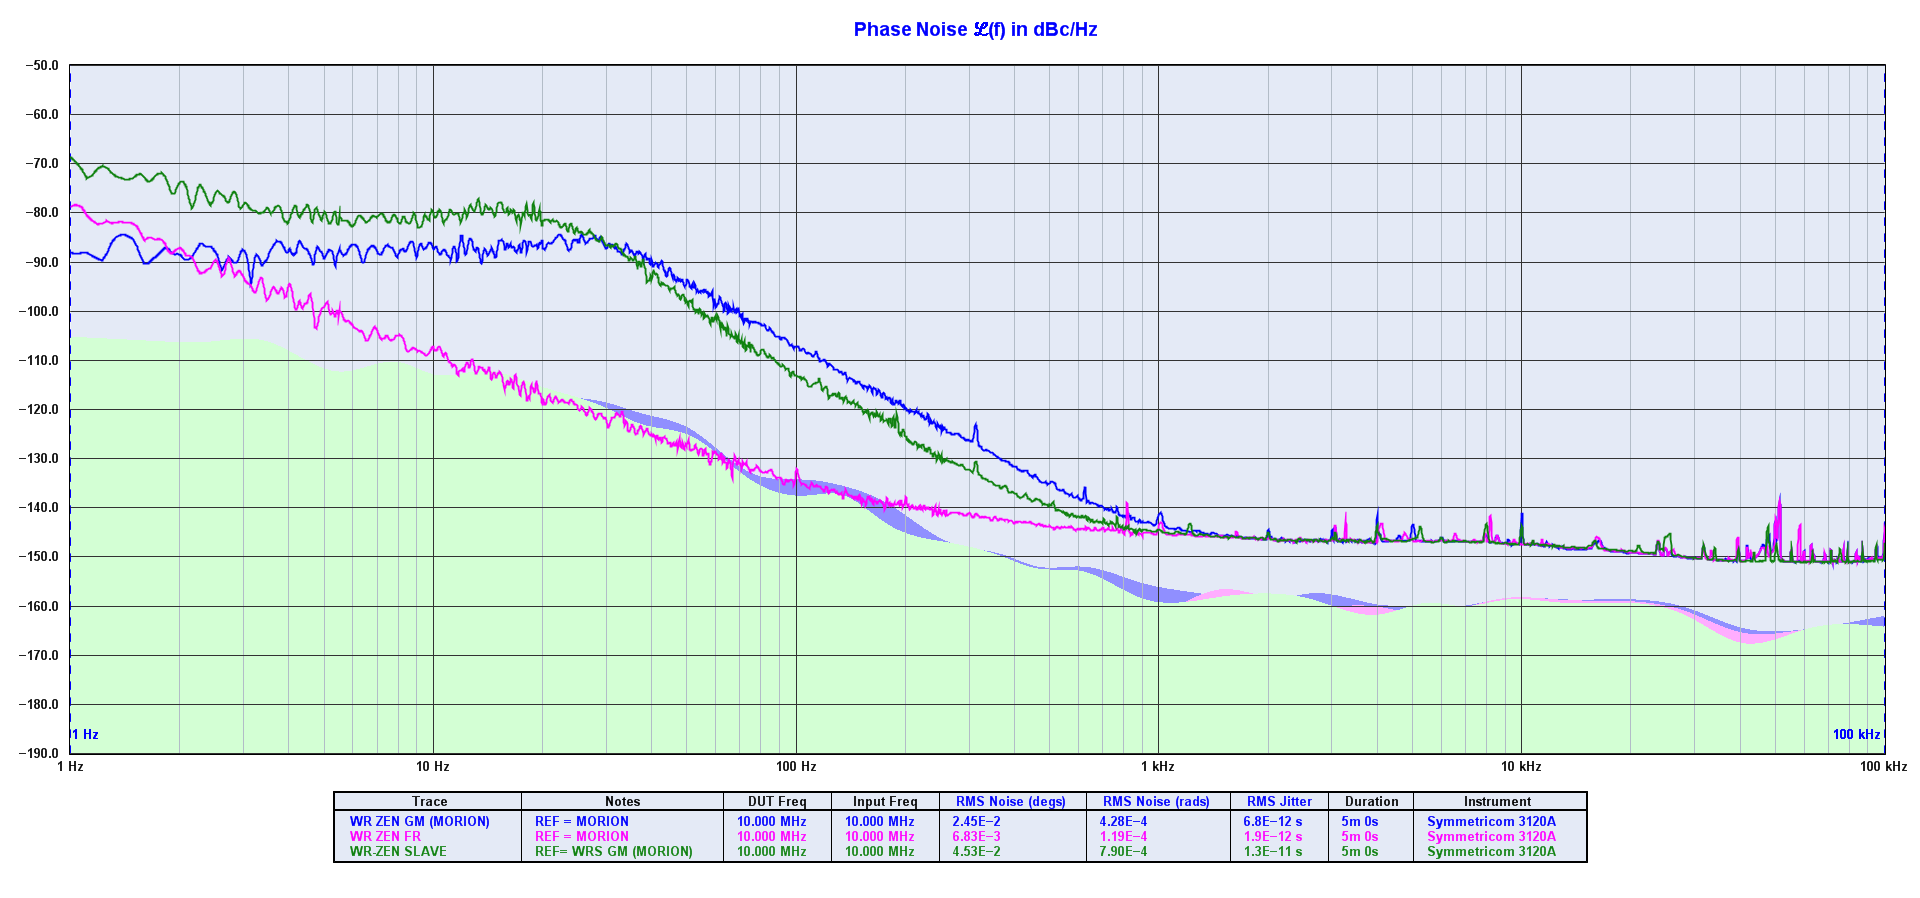
\includegraphics[width=\textwidth]{../measures/img/zen_all}
        \caption[Phase noise plot of the WR-ZEN]{The figure shows the Phase noise plot for the WR-ZEN in the Grand Master, Free Running and Slave modes. Sine wave output is compared to CMOS output.}
        \label{fig:zen_pn_all}
    \end{subfigure}
    ~ % This symbol adds a white space between images
    \begin{subfigure}[t]{0.45\textwidth}
         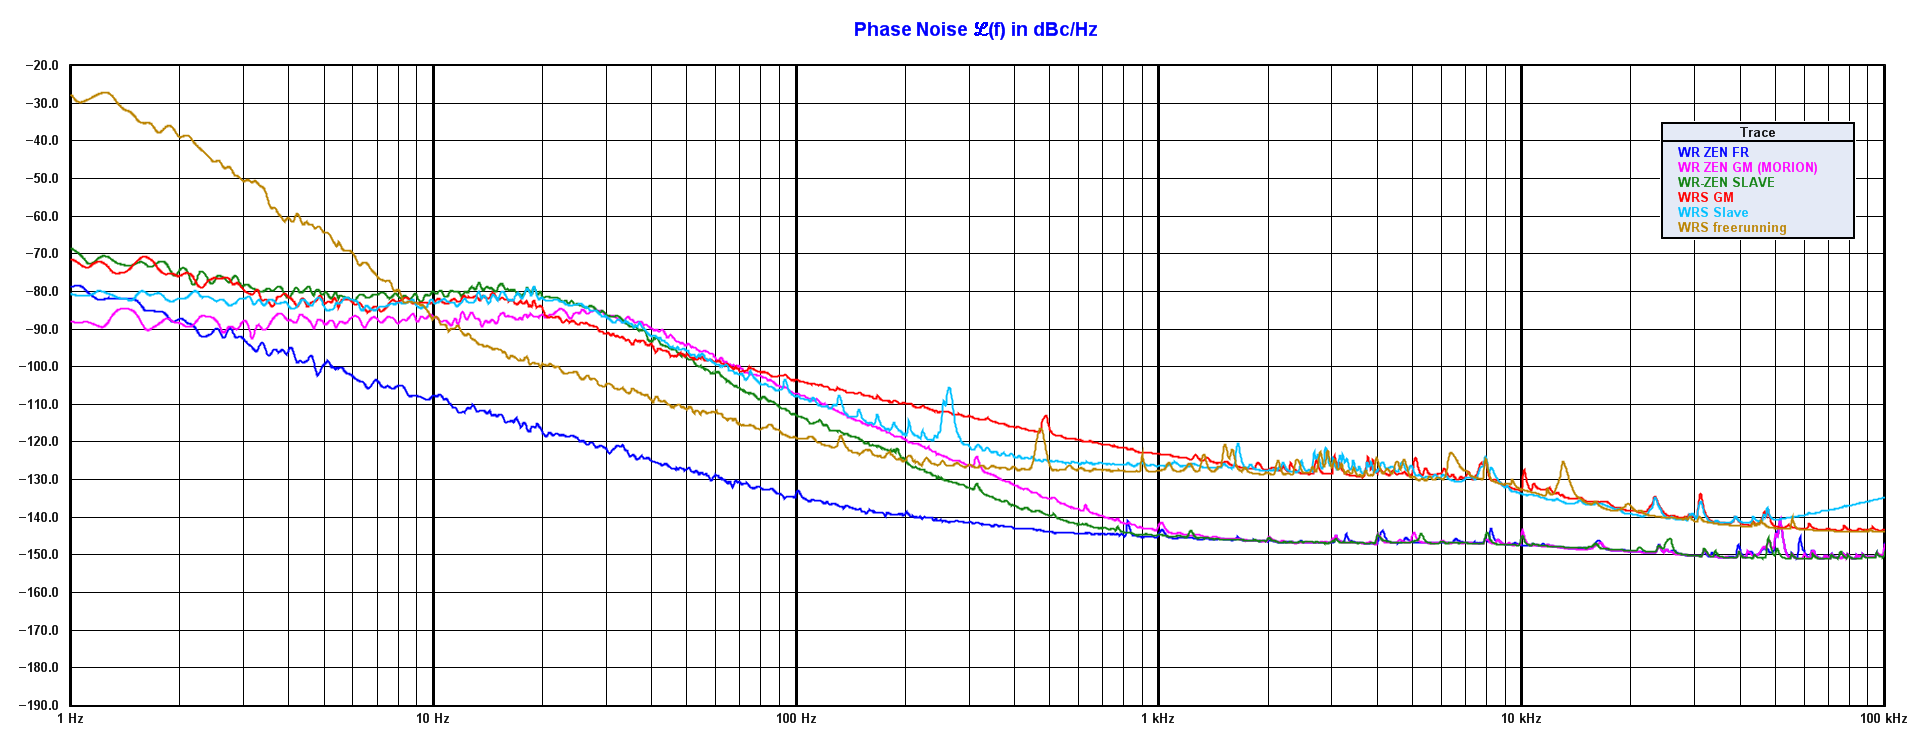
\includegraphics[width=\textwidth]{../measures/img/zen_vs_wrs}
         \caption[Phase noise plot of the WR-ZEN vs WRS]{The figure includes the same phase noise measures for the WRS. In this plot, only the CMOS outputs appear because the WRS doesn't have sine wave output signals.}
         \label{fig:zen_vs_wrs}
    \end{subfigure}
\end{figure}



It is also relevant to test the performance of the system when locking to an external reference in Grand master mode. Additive noise of the WR-ZEN will be propagated downstream, decreasing the quality of the Grand master's reference clock. It's very important that the system adds low noise in order to not degrade the quality of the external reference clock.

Results included in table \ref{tab:pn_results} ... \textcolor{blue}{TODO: hablar de la frecuencia de corte del softpll y del ddmtd.}

% \begin{table*}\centering
%     \ra{0.8}
%     \begin{tabular}{@{} rcccccc@{}}\toprule
%         & \multicolumn{4}{c}{Phase Noise (dBC/Hz)} & \phantom{} & \multirow{2}{*}{RMS Jitter}\\
%         \cmidrule(lr){2-5}
%         & @ 1 Hz & @ 20 Hz & @ 1 kHz  & @ 10 kHz && (ps)\\ \midrule
%         \textbf{Free running}\\
%         \small{WRS (CMOS)}             & -27.6 & -99.3  & -127.5 & -132.6 &&  620\\
%         \small{WR-ZEN (\textit{sine})} & -74.7 & -117.1 & -136.7 & -134.4 &&
%         2.5\\
%         \small{WR-ZEN (\textit{CMOS})} & -78.8 & -117.6 & -144.2 & -147.4 &&
%         1.9\\
%         
%         \textbf{Grand Master}\\
%         \small{WRS (CMOS)}             & -71.4 & -84.8  & -123.2 & -130.8 && 9.9\\
%         %\small{WR-ZEN (\textit{sine})} &  &  &  &  &&& \\
%         \small{WR-ZEN (\textit{CMOS})} & -88.1 & -86.3  & -141.9 & -144.1 && 6.8\\
%         
%         \textbf{Slave node}\\
%         \small{WRS (CMOS)}             & -80.7 & -81.9 & -126.2 & -133.8 &&  9.7\\
%         %\small{WR-ZEN (\textit{sine})} & -74.7 & -117.1 & -136.7 & -134.4 &&& 2.5 ps\\
%         \small{WR-ZEN (\textit{CMOS})} & -68.6 & -81.4 & -144.6 & -145.1 &&
%         13\\
%         
%         \bottomrule
%        \end{tabular}
%        \caption{Phase Noise results extracted from plots in figure \ref{fig:zen_pn_all} and \ref{fig:zen_vs_wrs}.}
%        \label{tab:pn_results}
%    \end{table*}
    
    
 \begin{table*}\centering
     \ra{0.8}
     \begin{tabular}{@{} rcccc@{}}%\toprule
         & \multicolumn{4}{c}{\bfseries{RMS jitter (ps)}} \\
         \cmidrule(l){2-5}
         & 1Hz-10Hz & 10Hz-1kHz & 1kHz-100kHz  & 1Hz-100kHz \\ \midrule
         \textbf{Free running}\\
         \small{WRS (CMOS)}             & 62  & 1.7  & 1.1  & 62  \\
         \small{WR-ZEN (\textit{sine})} & 2.1 & 0.24 & 1.4  & 2.5 \\
         \small{WR-ZEN (\textit{CMOS})} & 1.9 & 0.21 & 0.26 & 1.9 \\
         \cmidrule(l){2-5}
         
         \textbf{Grand Master}\\
         \small{WRS (CMOS)}             & 7.3 & 6.7 & 1.1 & 9.9\\
         \small{WR-ZEN (\textit{CMOS})} & 2.8 & 6.2 & 0.26 & 6.8\\
         \cmidrule(l){2-5}
         
         \textbf{Slave node}\\
         \small{WRS (CMOS)}             & 4.9 & 8.2 & 1.2  & 9.7\\
         \small{WR-ZEN (\textit{CMOS})} & 8.5 & 9.3 & 0.24 & 13\\
         
         \bottomrule
        \end{tabular}
        \caption{Phase Noise results extracted from plots in figure \ref{fig:zen_pn_all} and \ref{fig:zen_vs_wrs}.}
        \label{tab:pn_results}
\end{table*}

The slave mode results show that WR-ZEN performs slightly worse than WRS. Noise between 1 Hz and 20 Hz increases the RMS Jitter of the WR-ZEN. \textcolor{blue}{This may be caused by a poor adjustment of the PI control.}

\missingfigure{Allan deviation plot}

\subsection{Network experiment} %% Buscar un nombre mejor
\label{subsec: net_exp}

% Un experimento con una cadena de WRS y al final una ZEN

\subsection{Traffic influence on synchronization accuracy}

% Posible experimento metiendo tráfico a la cadena anterior

\subsection{Redundancy}

% Este no me queda muy claro, cuando toque se verá

\subsection{Thermal characterization...}

% Aquí irían el de la cámara térmica, mover las fibras para simular viento y
% chorradas por el estilo

 
